\documentclass[]{article}
\usepackage[utf8]{inputenc}
\usepackage[T1]{fontenc}
\usepackage[usenames,dvipsnames,pdftex]{xcolor}
\usepackage[upright]{fourier}
\usepackage[english]{babel}
\usepackage{hyperref}
\usepackage{calc}
\usepackage{amsmath}
\usepackage{amssymb}
\usepackage{mathrsfs}
\usepackage{amsthm}
\usepackage{fullpage}
\usepackage{tkz-graph}

\title{TP d'Algo/Complexité/Calculabilité}
\author{
  CIMBE Pierre-Alexandre \\
  LAGNIEZ Jean-Marc \\
  LESNYAK Viktor \\
  RAFIK Ahmed}
\date\today

\begin{document}

\makeatletter
  \begin{titlepage}
    \centering
        {\large \textsc{Université Montpellier II}}\\
        \textsc{Master 1ère Année Informatique}\\
        \vspace{1cm}
        
\includegraphics[width=0.25\textwidth]{logo.png}
        \hfill
        
\includegraphics[width=0.35\textwidth]{logo2.png}\\
        \vspace{1cm}
               {\large\textbf{	\@date\\
                   Rapport de Travaux Pratique}}\\
               \vfill
                   {\LARGE \textbf{\@title}} \\
                   \vspace{2em}
                          {\large \@author} \\
                          \vfill
  \end{titlepage}
\makeatother

%\maketitle

\section{Partie théorique}
\subsection{Partie algorithmique}

\subsubsection{Exercice 1}

\begin{enumerate}

\item Le nombre de s-t chemins d'arc disjoint est de 3.\\
On trouve ce résultat en appliquant l'algorithme de Ford-Fulkerson.\\
\begin{center}
s -> 4 -> 5 -> t      F = 1\\
s -> 3 -> 4 -> t      F = 1\\
s -> 2 -> 3 -> t      F = 1\\
\end{center}
Tous les arcs du graphe sont saturés donc on ne peut plus trouver de chemin améliorant et Fmax = 3.\\


\item Soit Si l'ensemble des sommets de la coupe i, $\overline Si$ l'ensemble des sommets du complémentaire de la coupe i, \\
Avi l'ensemble des arcs avants de la coupe i, et Ari l'ensemble des arcs arrière de cette coupe.\\
\begin{center}
S1 = \{1\} ; $\overline S1$ = \{2, 3, 4, 5, 6\}\\ 
Av1 = \{1->4 ; 1->3 ; 1->2\} ; Ar1 = \{\}\\
S2 = \{1, 2\} ; $\overline S2$ = \{3, 4, 5, 6\}\\
Av2 = \{1->4 ; 1->3 ; 2->3\} ; Ar2 = \{\}\\ 
S3 = \{1, 4\} ; $\overline S3$ = \{2, 3, 5, 6\}\\
Av3 = \{1->3 ; 1->2 ; 4->5 ; 4->6\} ; Ar3 = \{3->4\}\\
S4 = \{1, 2, 3\} ; $\overline S4$ = \{4, 5, 6\}\\ 
Av4 = \{1->4 ; 3->4 ; 3->6\} ; Ar4 = \{\}\\
S5 = \{1, 2, 4\} ; $\overline S5$ = \{3, 5, 6\}\\
Av5 = \{1->3 ; 2->3 ; 4->5 ; 4->6\} ; Ar5 = \{3->4\}\\
S6 = \{1, 4, 5\} ; $\overline S6$ = \{2, 3, 6\}\\
Av6 = \{1->2 ; 1->3 ; 4->6 ; 5->6\} ; Ar6 = \{3->4\}\\ 
S7 = \{1, 2, 3, 4\} ; $\overline S7$ = \{5, 6\}\\ 
Av7 = \{4->5 ; 4->6 ; 3->6\} ; Ar6 = \{\}\\ 
S8 = \{1, 2, 3, 4, 5\} ; $\overline S8$ = \{6\}\\
Av6 = \{3->6 ; 4->6 ; 5->6\} ; Ar6 = \{\}\\
\end{center}


\item Nombre minimum d'arc sortant dans une s-t coupe = 3\\
  Nombre maximum de chemin d'arc disjoint = 3\\

\end{enumerate}

\subsubsection{Exercice 2}

\textbf{Soit un graphe G=(V,E);\\avec $\forall i,j \in V$,\\
et f(i,j)-est la fonction représentant le flot de l'arc où $\forall (i,j)\in E$;\\}

\begin{enumerate}


\item Vrai, car si on enleve un arc (i,j), avec f(i,j)=0,\\ alors on n'influence pas la valeur du flot maximum.

\item Vrai, car dans un flot maximum, si un plus petit arc vital (i,j) n'a pas la plus petite valeur de f(i,j), alors il existe un arc (x,y) dans le flot maximum tel que f(x,y)<f(i,j). Par définition, l'arc (i,j) n'est donc pas le plus petit arc vital, ce qui est absurde.
\item Faux, voilà un contre exemple.


\usetikzlibrary{arrows}
\thispagestyle{empty}
\begin{center}
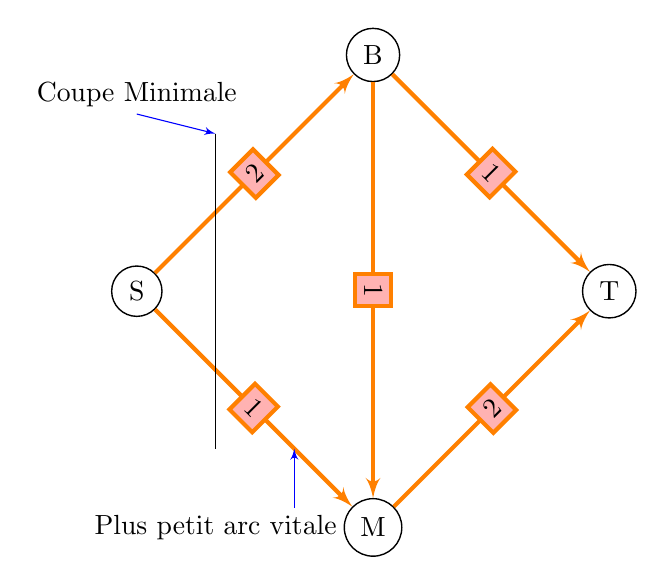
\begin{tikzpicture}[>=latex']
 \SetUpEdge[lw         = 1.5pt,
            color      = orange,
            labelcolor = red!30,
            labelstyle = {draw,sloped}]
  \tikzset{node distance = 5cm}
  \GraphInit[vstyle=Normal]
  \Vertex[x=-3, y=0]{S}
  \Vertex[x=0, y=3]{B}
  \Vertex[x=3, y=0]{T}
  \Vertex[x=0, y=-3]{M}
  \tikzset{EdgeStyle/.style={->}}
  \Edge[label=$2$](S)(B)
  \Edge[label=$1$](S)(M)
  \Edge[label=$1$](B)(T)
  \Edge[label=$2$](M)(T)
  \Edge[label=$1$](B)(M)
  \draw (-2,2) -- (-2,-2);
  \draw[blue,->](-1,-2.75)--(-1,-2);
  \draw[blue,->](-3,2.25)--(-2,2);

  \node at (-3,2.5){Coupe Minimale};
  \node at (-2,-3){Plus petit arc vitale};
\end{tikzpicture}
\end{center}
 
\end{enumerate} 

\subsubsection{Exercice 3}
Voici l'algorithme permettant de trouver une double étoile centrée de coût minimum centrée sur un sommet x dans le graphe G . On suppose que l'algorithme CouplageMin(Graphe A) permet d'obtenir un couplage de taille maximale et de coût minimal du graphe A. \\

Algorithme DoubleEtoileCentre(GrapheComplet G, Sommet x)\\
Retourne : Un sous-graphe de G isomorphe à une double-étoile centrée sur le sommet x de coût minimal.\\

Début\\
----Graphe G' = CouplageMin(G$\backslash$x);\\
----Pour chaque arête (i,j) de G':\\
--------Ajouter à G' l'arête de G de coût le plus faible entre l'arête (x,i) et l'arête (x,j);\\
--------/*Cette étape n'est possible que parce-que le graphe est complet.*/\\
----Fin pour\\
Fin\\

Il suffit ensuite d'appliquer cet algorithe à tous les sommets du graphe G et de garder le graphe de coût total le plus petit.

Algorithme DoubleEtoile(GrapheComplet G)\\
Retourne : Un sous-graphe de G isomorphe à une double-étoile de coût minimal.\\

Début\\
----Graphe G';\\
----Pour chaque sommet s de G:\\
--------G''= DoubleEtoileCentre(G, s);\\
--------Comparer le coût total de G'' à celui de G';\\
--------Si le coût de G'' est inférieur au coût de G', alors G' = G'';\\
----Fin pour\\
----Renvoyer G';\\
Fin\\

\subsubsection{Exercie 4}

\begin{enumerate}
\item Déroulement de l'algorithme :
\usetikzlibrary{arrows}
\begin{center}
Graphe initial\\
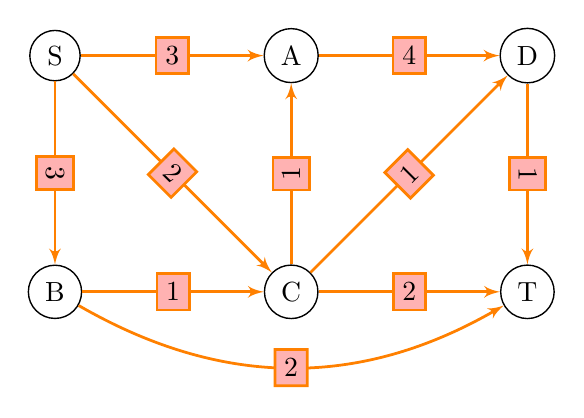
\begin{tikzpicture}[>=latex']
 \SetUpEdge[lw         = 1pt,
            color      = orange,
            labelcolor = red!30,
            labelstyle = {draw,sloped}]
  \tikzset{node distance = 2cm}
  \GraphInit[vstyle=Normal]
  \Vertex[x=-3, y=3]{S}
  \Vertex[x=0, y=3]{A}
  \Vertex[x=3, y=3]{D}
  \Vertex[x=3, y=0]{T}
  \Vertex[x=0, y=0]{C}
  \Vertex[x=-3, y=0]{B}
  \tikzset{EdgeStyle/.style={->}}
  \Edge[label=$3$](S)(B)
  \Edge[label=$2$](S)(C)
  \Edge[label=$3$](S)(A)
  \Edge[label=$2$](C)(T)
  \Edge[label=$1$](D)(T)
  \Edge[label=$4$](A)(D)
  \Edge[label=$1$](C)(A)
  \Edge[label=$1$](C)(D)
  \Edge[label=$1$](B)(C)
  \tikzset{EdgeStyle/.style={->}, bend right}
  \Edge[label=$2$](B)(T)
\end{tikzpicture}
\end{center}
\begin{enumerate}
\item Première phase : $\Delta = 2^{[\log(C)]} = 4$ \\

\begin{center}
Graphe résiduel $G(f,\Delta)$\\
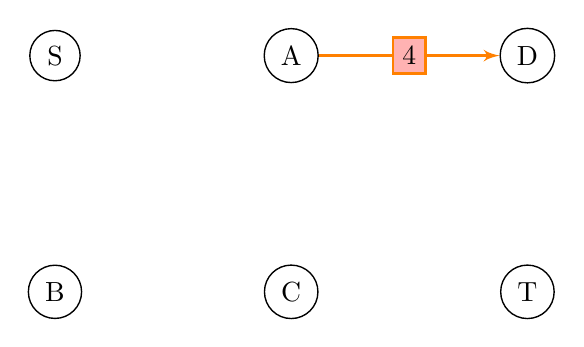
\begin{tikzpicture}[>=latex']
 \SetUpEdge[lw         = 1pt,
            color      = orange,
            labelcolor = red!30,
            labelstyle = {draw,sloped}]
  \tikzset{node distance = 2cm}
  \GraphInit[vstyle=Normal]
  \Vertex[x=-3, y=3]{S}
  \Vertex[x=0, y=3]{A}
  \Vertex[x=3, y=3]{D}
  \Vertex[x=3, y=0]{T}
  \Vertex[x=0, y=0]{C}
  \Vertex[x=-3, y=0]{B}
  \tikzset{EdgeStyle/.style={->}}
  \Edge[label=$4$](A)(D)
  \tikzset{EdgeStyle/.style={->}, bend right}
\end{tikzpicture}
\end{center}

Pas de chemin de s à p, $\Delta = \Delta/2$\\

\item Seconde phase : $\Delta = 2$ \\

\begin{center}
Graphe résiduel $G(f,\Delta)$\\
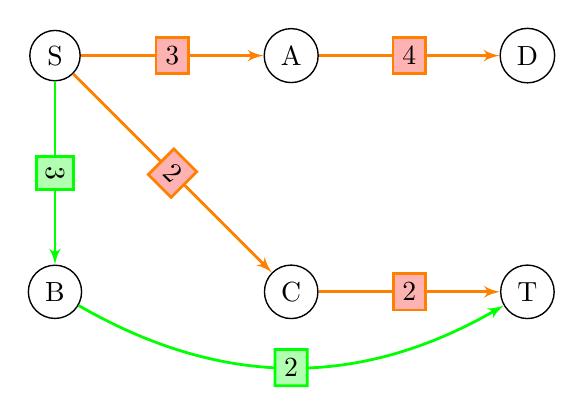
\begin{tikzpicture}[>=latex']
 \SetUpEdge[lw         = 1pt,
            color      = orange,
            labelcolor = red!30,
            labelstyle = {draw,sloped}]
  \tikzset{node distance = 2cm}
  \GraphInit[vstyle=Normal]
  \Vertex[x=-3, y=3]{S}
  \Vertex[x=0, y=3]{A}
  \Vertex[x=3, y=3]{D}
  \Vertex[x=3, y=0]{T}
  \Vertex[x=0, y=0]{C}
  \Vertex[x=-3, y=0]{B}
  \tikzset{EdgeStyle/.style={->}}
  \Edge[label=$3$,color=green,labelcolor=green!30](S)(B)
  \Edge[label=$2$](S)(C)
  \Edge[label=$3$](S)(A)
  \Edge[label=$2$](C)(T)
  \Edge[label=$4$](A)(D)
  \tikzset{EdgeStyle/.style={->}, bend right}
  \Edge[label=$2$,color=green,labelcolor=green!30](B)(T)
\end{tikzpicture}
\end{center}


Premier chemin :\\
$s \rightarrow b \rightarrow t$  \\
$\delta = 2$  \\
$F = 2$\\

\begin{center}
\vspace*{7mm}
Graphe résiduel $G(f,\Delta)$\\
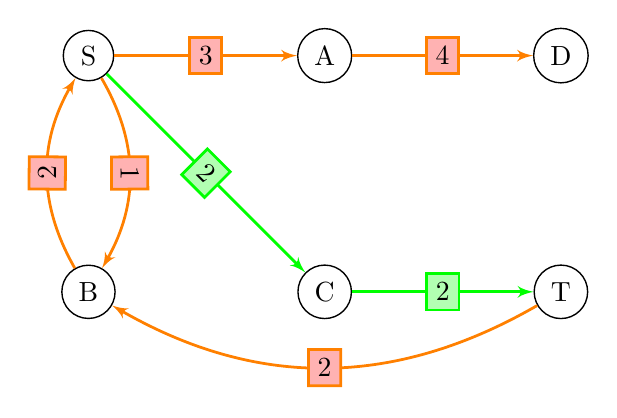
\begin{tikzpicture}[>=latex']
 \SetUpEdge[lw         = 1pt,
            color      = orange,
            labelcolor = red!30,
            labelstyle = {draw,sloped}]
  \tikzset{node distance = 2cm}
  \GraphInit[vstyle=Normal]
  \Vertex[x=-3, y=3]{S}
  \Vertex[x=0, y=3]{A}
  \Vertex[x=3, y=3]{D}
  \Vertex[x=3, y=0]{T}
  \Vertex[x=0, y=0]{C}
  \Vertex[x=-3, y=0]{B}
  \tikzset{EdgeStyle/.style={->}}
  \Edge[label=$2$,color=green,labelcolor=green!30](S)(C)
  \Edge[label=$3$](S)(A)
  \Edge[label=$2$,color=green,labelcolor=green!30](C)(T)
  \Edge[label=$4$](A)(D)
  \tikzset{EdgeStyle/.style={->}, bend left}
  \Edge[label=$2$](T)(B)
  \Edge[label=$2$](B)(S)
  \Edge[label=$1$](S)(B)
\end{tikzpicture}
\end{center}
\vspace*{7mm}
Second chemin :\\
$s \rightarrow c \rightarrow t$  \\
$\delta = 2$  \\
$F = 4$\\

\begin{center}
Graphe résiduel $G(f,\Delta)$\\
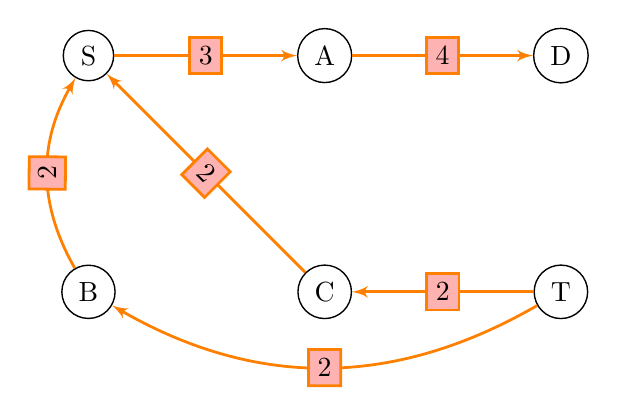
\begin{tikzpicture}[>=latex']
 \SetUpEdge[lw         = 1pt,
            color      = orange,
            labelcolor = red!30,
            labelstyle = {draw,sloped}]
  \tikzset{node distance = 2cm}
  \GraphInit[vstyle=Normal]
  \Vertex[x=-3, y=3]{S}
  \Vertex[x=0, y=3]{A}
  \Vertex[x=3, y=3]{D}
  \Vertex[x=3, y=0]{T}
  \Vertex[x=0, y=0]{C}
  \Vertex[x=-3, y=0]{B}
  \tikzset{EdgeStyle/.style={->}}
  \Edge[label=$2$](C)(S)
  \Edge[label=$2$](T)(C)
  \Edge[label=$3$](S)(A)
  \Edge[label=$4$](A)(D)
   \tikzset{EdgeStyle/.style={->}, bend left}
  \Edge[label=$2$](T)(B)
  \Edge[label=$2$](B)(S)
\end{tikzpicture}
\end{center}

Pas d'autre chemin dans le graphe. $\Delta = \Delta/2$\\

\item Troisième phase : $\Delta = 1$ \\

\begin{center}
Flot actuel au début de cette phase :\\
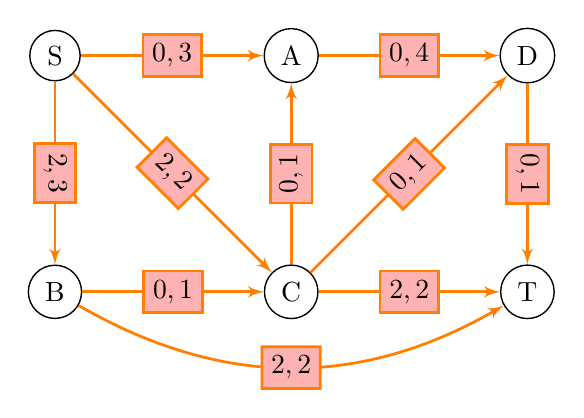
\begin{tikzpicture}[>=latex']
 \SetUpEdge[lw         = 1pt,
            color      = orange,
            labelcolor = red!30,
            labelstyle = {draw,sloped}]
  \tikzset{node distance = 2cm}
  \GraphInit[vstyle=Normal]
  \Vertex[x=-3, y=3]{S}
  \Vertex[x=0, y=3]{A}
  \Vertex[x=3, y=3]{D}
  \Vertex[x=3, y=0]{T}
  \Vertex[x=0, y=0]{C}
  \Vertex[x=-3, y=0]{B}
  \tikzset{EdgeStyle/.style={->}}
  \Edge[label=${2,3}$](S)(B)
  \Edge[label=${2,2}$](S)(C)
  \Edge[label=${0,3}$](S)(A)
  \Edge[label=${2,2}$](C)(T)
  \Edge[label=${0,1}$](D)(T)
  \Edge[label=${0,4}$](A)(D)
  \Edge[label=${0,1}$](C)(A)
  \Edge[label=${0,1}$](C)(D)
  \Edge[label=${0,1}$](B)(C)
  \tikzset{EdgeStyle/.style={->}, bend right}
  \Edge[label=${2,2}$](B)(T)
\end{tikzpicture}
\end{center}
\vspace*{7mm}
\begin{center}
Graphe résiduel $G(f,\Delta)$\\
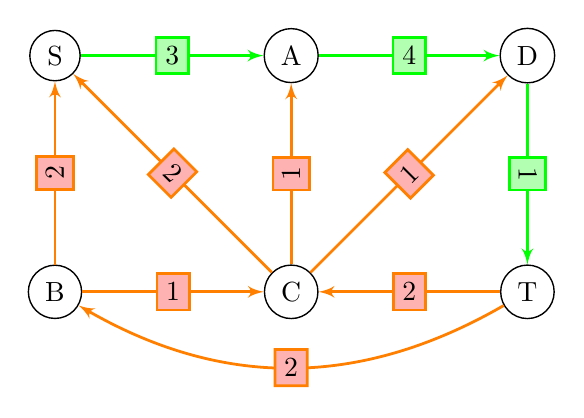
\begin{tikzpicture}[>=latex']
 \SetUpEdge[lw         = 1pt,
            color      = orange,
            labelcolor = red!30,
            labelstyle = {draw,sloped}]
  \tikzset{node distance = 2cm}
  \GraphInit[vstyle=Normal]
  \Vertex[x=-3, y=3]{S}
  \Vertex[x=0, y=3]{A}
  \Vertex[x=3, y=3]{D}
  \Vertex[x=3, y=0]{T}
  \Vertex[x=0, y=0]{C}
  \Vertex[x=-3, y=0]{B}
  \tikzset{EdgeStyle/.style={->}}
  \Edge[label=$2$](C)(S)
  \Edge[label=$2$](T)(C)
  \Edge[label=$3$,color=green,labelcolor=green!30](S)(A)
  \Edge[label=$4$,color=green,labelcolor=green!30](A)(D)
  \Edge[label=$1$,color=green,labelcolor=green!30](D)(T)
  \Edge[label=$1$](C)(A)
  \Edge[label=$1$](C)(D)
  \Edge[label=$1$](B)(C)
  \Edge[label=$2$](B)(S)
  \tikzset{EdgeStyle/.style={->}, bend left}
  \Edge[label=$2$](T)(B)
\end{tikzpicture}
\end{center}

Premier chemin :\\
$s \rightarrow a \rightarrow d \rightarrow t$  \\
$\delta = 1$  \\
$F = 5$\\

\vspace*{7mm}
\begin{center}
Graphe résiduel $G(f,\Delta)$\\
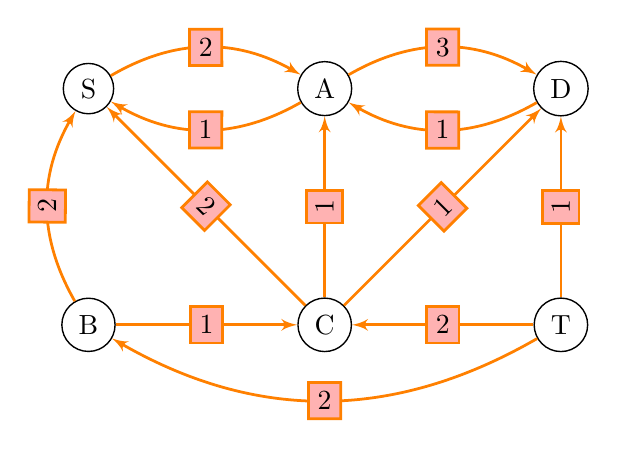
\begin{tikzpicture}[>=latex']
 \SetUpEdge[lw         = 1pt,
            color      = orange,
            labelcolor = red!30,
            labelstyle = {draw,sloped}]
  \tikzset{node distance = 2cm}
  \GraphInit[vstyle=Normal]
  \Vertex[x=-3, y=3]{S}
  \Vertex[x=0, y=3]{A}
  \Vertex[x=3, y=3]{D}
  \Vertex[x=3, y=0]{T}
  \Vertex[x=0, y=0]{C}
  \Vertex[x=-3, y=0]{B}
  \tikzset{EdgeStyle/.style={->}}
  \Edge[label=$2$](C)(S)
  \Edge[label=$2$](T)(C)
  \Edge[label=$1$](T)(D)
  \Edge[label=$1$](C)(A)
  \Edge[label=$1$](C)(D)
  \Edge[label=$1$](B)(C)
  \tikzset{EdgeStyle/.style={->}, bend left}
  \Edge[label=$2$](T)(B)
  \Edge[label=$2$](B)(S)
  \Edge[label=$2$](S)(A)
  \Edge[label=$3$](A)(D)
  \Edge[label=$1$](A)(S)
  \Edge[label=$1$](D)(A)
\end{tikzpicture}
\end{center}
Pas d'autre chemin dans le graphe. L'algorithme est terminé.\\
\item Flot maximum $F=5$\\
\begin{center}
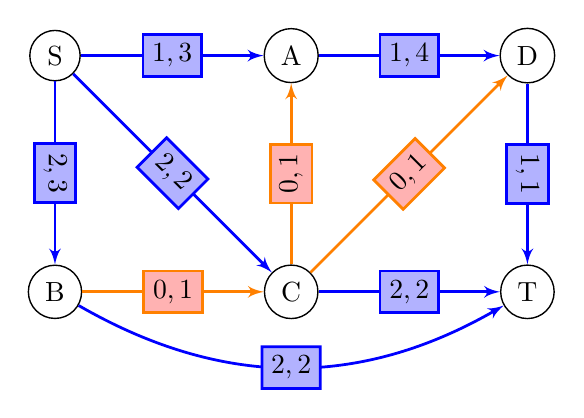
\begin{tikzpicture}[>=latex']
 \SetUpEdge[lw         = 1pt,
            color      = orange,
            labelcolor = red!30,
            labelstyle = {draw,sloped}]
  \tikzset{node distance = 2cm}
  \GraphInit[vstyle=Normal]
  \Vertex[x=-3, y=3]{S}
  \Vertex[x=0, y=3]{A}
  \Vertex[x=3, y=3]{D}
  \Vertex[x=3, y=0]{T}
  \Vertex[x=0, y=0]{C}
  \Vertex[x=-3, y=0]{B}
  \tikzset{EdgeStyle/.style={->}}
  \Edge[label=${2,3}$,color=blue,labelcolor=blue!30](S)(B)
  \Edge[label=${2,2}$,color=blue,labelcolor=blue!30](S)(C)
  \Edge[label=${1,3}$,color=blue,labelcolor=blue!30](S)(A)
  \Edge[label=${2,2}$,color=blue,labelcolor=blue!30](C)(T)
  \Edge[label=${1,1}$,color=blue,labelcolor=blue!30](D)(T)
  \Edge[label=${1,4}$,color=blue,labelcolor=blue!30](A)(D)
  \Edge[label=${0,1}$](C)(A)
  \Edge[label=${0,1}$](C)(D)
  \Edge[label=${0,1}$](B)(C)
  \tikzset{EdgeStyle/.style={->}, bend right}
  \Edge[label=${2,2}$,color=blue,labelcolor=blue!30](B)(T)
\end{tikzpicture}
\end{center}
\end{enumerate}
\vspace*{7mm}
\item \\
\begin{enumerate}
\item A la fin d'une phase, il n'y a plus de chemin de s à t, donc $t\notin S$.\\
On peut en déduire que $[S,\overline{S}]$ est une s-t coupe.
\vspace*{7mm}
\item La valeur de la capacité résiduelle maximum est 0.\\
Preuve par l'absurde: $\forall i\in S,j \in \overline{S}$, si $(i,j)$ existe, alors $j$ est atteignable par $i$, donc par $s$, donc $j\in S$.\\
Il y a au plus m arêtes dans la coupe, chacune ayant un coût maximal égal à $2\Delta$ , soit la valeur de $\Delta$ à l'étape précédente. Donc $C(S,\overline{S})\le 2\Delta m$.
\vspace*{7mm}
\item Une s-t coupe dans le graphe $G(f',\Delta)$ correspond au flot maximum que l'on peut encore ajouter à F. Or, comme précédemment dit, la coupe $[S,\overline{S}]$ est une s-t coupe. Donc on ne peut augmenter f' qu'au maximum de $2 \Delta m$, donc $f^*\le f'+2 \Delta m \leftrightarrow f^* - f' \le 2 \Delta m$.
\vspace*{7mm}
\item Lors de la phase suivante, chaque augmentation est majorée par $\Delta$ (soit $2*\Delta /2$). Il y a donc $2\Delta m / \Delta = 2m$ augmentations par phase au maximum.\\
\end{enumerate}
\vspace*{7mm}
\item Il y a $log C$ phases.\\

\item La recherche d'un chemin améliorant est en $O(m)$. Le nombre d'augmentations effectuées au total est en $O(m log C)$. Donc l'algorithme admet une complexité de $O(m^2log C)$.\\
\end{enumerate}

\subsection{Partie complexité}

\subsubsection{Exercie 5}

\begin{enumerate}
\item 
  \begin{enumerate}
  \item
    SAT : Un  problème SAT est un problème de décision visant à montrer l'existence d'une interprétation satisfaisant un ensemble de variables propositionnelles (Formule logique CNF)\\
    3-SAT : Cas particulier du problème SAT dans lequel les clauses sont toutes de taille 3.\\

  \item
    On dit qu'il existe une réduction d'un problème P à un problème P' s'il existe une fonction f\\
    telle que x $\in$ D(P) <=> f(x) $\in$ D(P')\\

  \item
    3-SAT est un cas particulier de SAT, or SAT $\in$ NP.\\
    Donc 3-SAT $\in$ NP

    SAT $\in$ NP-Complet

    Nous allons chercher à réduire un problème SAT à un problème 3-SAT : 

    Soit P une instance du problème SAT.
    
    $\twoheadrightarrow$Soit U=($l_1 \vee l_2 \vee l_3......\vee l_k$) une clause de taille k > 3

    On la divise en 2 clause :
    $\succ$ une clause de taille $\lfloor$k/2$\rfloor$+1 en complétant par une variable x$\notin$U 
    $\succ$ une clause de taille $\lceil$k/2$\rceil$+1 en complétant par $\overline x$ le complémentaire de x.

    On applique ce principe récursivement jusqu'à obtenir des clauses de taille 3

    $\twoheadrightarrow$Soit U={$l_1 \vee l_2$} une clause de taille 2
    
    On clone la clause U pour avoir 2 clauses $U_1$ et $U_2$ auxquelles on ajoute respectivement une variable x et son complémentaire $\overline x$
    on obtient :  $U_1$={$l_1 \vee l_2$vx}
    $U_2$={$l_1 \vee l_2 \vee \overline x$}

    $\twoheadrightarrow$Soit U={$l_1$} une clause de taille 1
    On force $l_1$ à vrai et on retire les clauses unitaires.

    On obtient ainsi un problème P' de type 3-SAT.    

    Donc 3-SAT est NP-Complet.\\

    \item
      Détaillons chaque cas concernant chaque type de clause :
     $\twoheadrightarrow$\underline{Clause de taille 4 :}\\
     Soit ($l_1 \vee l_2 \vee l_3 \vee l_4$) une clause de taille 4\\

      \begin{center}
        $(l_1 \vee l_2 \vee l_3 \vee l_4)\left\lbrace 
        \begin{array}{lcl} 
          (l_1 \vee l_2 \vee u)\\ 
          (l_3 \vee l_4 \vee \overline u)\\ 
        \end{array}\right.$ 
      \end{center}

      Chaque clause contenant 4 littéraux est ainsi divisée en 2 clauses de 3 littéraux
      \begin{center}
        $n_4$ -> 2$n_4$
      \end{center}
      On ajoute ainsi une variable pour chaque clause
      \begin{center}
        4$n_4$ -> 5$n_4$
      \end{center}
      \bigbreak

      $\twoheadrightarrow$\underline{Clause de taille 5 :}\\      
      Soit ($l_1 \vee l_2 \vee l_3 \vee l_4 \vee l_5$) une clause de taille 5

      \begin{center}
     $ (l_1 \vee l_2 \vee l_3 \vee l_4 \vee l_5)\left\lbrace
      \begin{array}{lcl}
        (l_1 \vee l_2 \vee u)\\
        (l_3 \vee l_4 \vee l_5 \vee \overline u)
      \end{array}\right.$
      \end{center}

      \begin{center}
        $(l_3 \vee l_4 \vee l_5 \vee \overline u)\left\lbrace
      \begin{array}{lcl} 
        (l_3 \vee l_4 \vee y)\\
        (l_5 \vee \overline u \vee \overline y)
      \end{array}\right.$
      \end{center}

      Chaque clause contenant 5 littéraux est ainsi divisée en 3 clauses de 3 littéraux
      \begin{center}
        $n_5$ -> 3$n_5$
      \end{center}
      On ajoute ainsi 2 variables pour chaque clause
      \begin{center}
        5$n_5$ -> 7$n_5$
      \end{center}
      \bigbreak

      $\twoheadrightarrow$\underline{Clause de taille 2 :}\\
      Soit ($l_1 \vee l_2$) une clause de taille 2

      \begin{center}
      $(l_1 \vee l_2)\left\lbrace
      \begin{array}{lcl} 
        (l_1 \vee l_2 \vee u)\\
        (l_1 \vee l_2 \vee \overline u)
      \end{array}\right.$
      \end{center}

      Chaque clause contenant 2 littéraux est transformée en 2 clauses de 3 littéraux
      \begin{center}
        $n_2$ -> 2$n_2$
      \end{center}
      On ajoute ainsi 1 variables pour chaque clause
      \begin{center}
        2$n_2$ -> 3$n_2$
      \end{center}
      \bigbreak


      $\twoheadrightarrow$\underline{Clause de taille 1 :}\\
      Soit ($l_1$) une clause de taille 1

      \begin{center}
      $(l_1)\left\lbrace 
      \begin{array}{lcl} 
        (l_1 \vee u \vee \overline u)
      \end{array}\right.$
      \end{center}

      Chaque clause contenant 1 littéraux est transformée en une clause de 3 littéraux
      \begin{center}
        $n_1$ -> $n_1$
      \end{center}
      On ajoute ainsi 1 variables pour chaque clause
      \begin{center}
        $n_1$ -> 3$n_1$
      \end{center}
      \bigbreak

      On peut donc conclure :
      \begin{center}
        Nombre de clauses = $n_1 + 3n_2 + n_3 + 2n_4 + 3n_5$\\
        Nombre de variables = $3n_1 + 3n_2 + 3n_3 + 5n_4 + 7n_5$\\
      \end{center}
      \bigbreak

\end{enumerate}
  
  \item
    Soit U = ($l_1 \vee l_2 \vee l_3$) une clause de taille 3\\
    \smallbreak
    En appliquant la réduction, on obtient :\\
    
    \begin{center}
      $(l_1 \vee l_2 \vee l_3)\left\lbrace 
      \begin{array}{lcl}
        (l_1 \vee u)\\
        (l_2 \vee l_3 \vee \overline u)
      \end{array}\right.$
    \end{center}
    \smallbreak

    On obtient ainsi une nouvelle clause de taille 3.\\
    Il est donc impossible de réduire un problème 3-SAT à un problème 2-SAT de cette manière.\\
    \smallbreak

    \item
    \smallbreak

    \item
      \begin{enumerate}
        \item
          Le problème étudié fait évidement partie de la classe NP.\\
          En effet, on vérifie aisement, à partir d'un ensemble L de sommets, que L est l'ensemble des feuilles d'un arbre couvrant de G.\\

          Réduction :
          Soit un graphe G = (V,E) et un ensemble L $\subset$ V.\\
          On choisis arbitrairement 2 sommets x et y dans L.  \\        
          On prend le sous graphe G' = (V',E') tel que V'={V-{L-{x,y}}}\\
          

          Si il existe un chemin Hamiltonien entre x et y dans G' alors il existe un arbre couvrant dont l'ensemble des feuilles est L.\\
          En effet, le chemin hamiltonien relie tous les sommets de G'. En y rajoutant les sommets restant L on obtient un arbre couvrant de G.\\

          De la meme manière, si il existe un arbre couvrant dans G, on peut lui retirer les sommets de L-{x,y}. \\
          Ainsi il nous reste un chemin hamiltonien de x à y dans G'.\\

          Notre problème est donc NP-Complet.\\
          \smallbreak

        \item
          Le problème étudié fait évidement partie de la classe NP.\\
          En effet, on vérifie aisement, à partir d'un ensemble L de sommets, que l'ensemble des feuilles d'un arbre couvrant de G est contenu dans L.\\

          Réduction :
          Soit un graphe G = (V,E) et un ensemble L $\subset$ V.\\
          On choisit arbitrairement 2 sommets x et y dans L.  \\        
          On prend le sous graphe G' = (V',E') tel que V'={V-{L-{x,y}}}\\
          

          S'il existe un chemin Hamiltonien entre x et y dans G' alors il existe un arbre couvrant dont l'ensemble des feuilles est contenu L.\\

          S'il existe un arbre couvrant dans G, on peut lui retirer les sommets de L-{x,y}. \\
          Ainsi il nous reste un chemin hamiltonien de x à y dans G'.\\

          Notre problème est donc NP-Complet.\\

          \smallbreak
        \item
          

      \end{enumerate}
    \smallbreak
 
   \item
      Le problème Connected dominating fait évidement partie de la classe NP.\\
      En effet, on vérifie aisement, à partir d'un ensemble S, que chaque sommet x de G est soit dans S, soit un voisin d'un sommet de S.\\
      \smallbreak

      Réduction :
      Soit un graphe G(E,V) connexe.\\
      On crée un nouveau graphe G'(E',V') tel que $\forall$ (u,v)$\in$ E, on ajoute dans G' un nouveau sommet x relié à u et v.\\
      \smallbreak

      Un vertex cover de G est alors un ensemble dominant de G'.\\
      Donc, si on trouve un vertex cover de taille k dans G, alors $\exists$ S un ensemble dominant de taille k dans G' et inversement.\\
      \smallbreak

    \item
      Balanced 3-SAT est un cas particulier de Balanced SAT, or Balanced SAT $\in$ NP.\\
      Donc Balanced 3-SAT $\in$ NP\\

      Balanced SAT $\in$ NP-Complet\\

      On réduit balanced SAT à balanced 3-SAT de la même manière que nous avons réduit SAT à 3-SAT.\\
      Nous savons que balanced SAT est NP-Complet donc balanced 3-SAT est NP-Complet.\\

\end{enumerate}

\subsubsection{Exercice 6}

\begin{enumerate}
\item 
\begin{enumerate}
\item Un sommet isolé ne couvre aucun arc et n'apparaît dans aucun vertex-cover de G. En retirant ce sommet, on réduit à n-1 la taille du graphe sans affecter la solution.\\
\item Un sommet de degré 1 ne couvre qu'une seule arête, cette même arête étant couverte par son voisin y. Tout vertex-cover de G contient soit x, soit y. y couvrant au moins autant d'arêtes que x, il appartient à une solution optimale du problème. En supprimant y de G, on réduit le problème à une taille n-1 et un paramètre k-1.\\
\item Si G possède une solution de taille k et qu'un sommet x de degré supérieur à k n'appartient pas à cette solution, alors tous les voisins de x appartiennent à cette solution. Ceci est absurde car x possède au moins k+1 voisins. Tout sommet x de degré supérieur à k appartient donc à une solution optimale de taille k si celle-ci existe. 
\end{enumerate}
\item
\begin{enumerate}
\item On sait, après kernelization du problème, que tous les sommets restant dans le graphe réduit sont de degré maximum k. Si G' possède une solution de taillek, alors les k sommets de la solution couvrent au plus k arêtes chacun, soit k² arêtes.\\
\item De la même manière, si G' possède une solution de taille k, alors les k sommets de la solution possèdent au plus k voisins chacun. Le graphe réduit possède alors k²+k sommets au maximum, soit les k sommets de la solution et leurs k² voisins.\\
\end{enumerate}
\item 
\begin{enumerate}
\item Soit un graphe réduit G' possédant au moins k²+1 arêtes. Si G' possède une solution de taille k, alors l'un de  ces k sommets est au moins de degré k+1. Donc G' n'est pas un graphe réduit, ce qui est absurde.\\
\item Soit G' un graphe réduit possédant au moins k²+k+1 sommets. Si G' possède une solution de taille k, alors l'un des k sommets de la solution est de degré supérieur ou égal à k+1, ou il existe au moins un sommet isolé. Dans les deux cas, G' n'est pas un graphe réduit, ce qui est absurde.
\end{enumerate}
\vspace*{7mm}
\item
\begin{enumerate}
\item
\begin{enumerate}
\item Preuve de terminaison : La condition de sortie de la récursion est basée sur deux paramètres k et $|E(G)|$. A chaque appel récursif, k décroît strictement. Le nombre d'appel récursif est donc borné par k, l'algorithme s'arrête donc à coup sûr.\\
\item Preuve de conformité du résultat : \\

Si VC(G,k) = vrai :\\
Notons C son vertex-cover. \\
Soit une arête {u,v} tel que $u\in C$ ou $v\in C$.\\
Si $u\in C$, alors $C\backslash{u}$ est un vertex-cover de $G\backslash{u}$ de taille k-1.\\
$VC(G\backslash{u}, k-1)$ est donc vrai.\\
De même pour v, on a donc bien $VC(G1,k-1)\vee VC(G2,k-1)$ = vrai.\\

Si VC(G,k) = faux :\\
$G\backslash{u}$ et $G\backslash{v}$ ne peuvent pas avoir de vertex-cover de taille k-1 puisque G n'a pas de vertex-cover de taille k. $VC(G1,k-1) = VC(G2,k-1)$ = faux;\\
Donc on a bien $VC(G1,k-1)\vee VC(G2,k-1)$ = faux.\\
On peut donc conclure que $VC(G,k) = VC(G1,k-1)\vee VC(G2,k-1)$ quelque-soit k.\\
\end{enumerate}
\item Dans le pire des cas, l'algorithme s'arrête lorsque k=0. Donc on effectue k itérations, chacune ayant une complexité bornée par le coût de construction des deux sous-graphes, soit $O(n^2)$. L'algorithme a donc une complexité en $O(n^{2k})$.\\
\end{enumerate}
\item Déroulement de la méthode :\\
\begin{enumerate}
\item 
VC(G1,3)=vrai\\
\begin{enumerate}
\item Graphe G1
\begin{center}
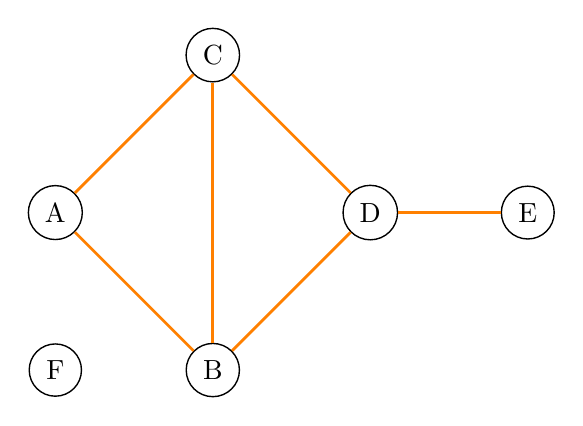
\begin{tikzpicture}[>=latex']
 \SetUpEdge[lw         = 1pt,
            color      = orange,
            labelcolor = red!30,
            labelstyle = {draw,sloped}]
  \tikzset{node distance = 2cm}
  \GraphInit[vstyle=Normal]
  \Vertex[x=-3, y=0]{A}
  \Vertex[x=-1, y=-2]{B}
  \Vertex[x=-1, y=2]{C}
  \Vertex[x=1, y=0]{D}
  \Vertex[x=3, y=0]{E}
  \Vertex[x=-3, y=-2]{F}
  \tikzset{EdgeStyle/.style={-}}
  \Edge[](A)(B)
  \Edge[](A)(C)
  \Edge[](B)(C)
  \Edge[](C)(D)
  \Edge[](B)(D)
  \Edge[](D)(E)
\end{tikzpicture}
\end{center}
\vspace*{7mm}
\item Réductions :\\
\vspace*{7mm}
\begin{center}
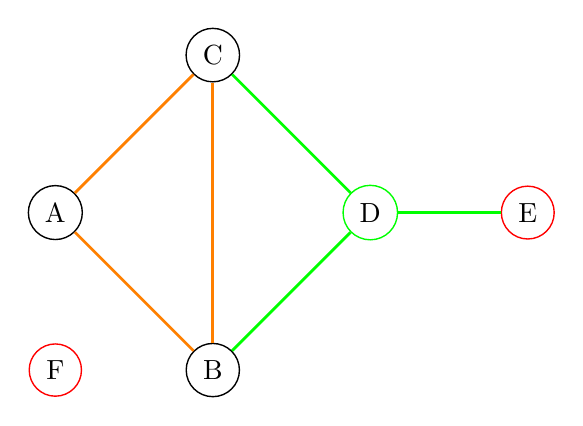
\begin{tikzpicture}[>=latex']
 \SetUpEdge[lw         = 1pt,
            color      = orange,
            labelcolor = red!30,
            labelstyle = {draw,sloped}]
  \tikzset{node distance = 2cm}
  \GraphInit[vstyle=Normal]
  \Vertex[x=-3, y=0]{A}
  \Vertex[x=-1, y=-2]{B}
  \Vertex[x=-1, y=2]{C}
  \begin{scope}[VertexStyle/.append style = {draw=green}]
  \Vertex[x=1, y=0]{D}
  \end{scope}
  \begin{scope}[VertexStyle/.append style = {draw=red}]
  \Vertex[x=3, y=0]{E}
  \Vertex[x=-3, y=-2]{F}
  \end{scope}
  \tikzset{EdgeStyle/.style={-}}
  \Edge[](A)(B)
  \Edge[](A)(C)
  \Edge[](B)(C)
  \Edge[color=green](C)(D)
  \Edge[color=green](B)(D)
  \Edge[color=green](D)(E)
\end{tikzpicture}
\end{center}
\vspace*{7mm}
E est un sommet de degré 1. On le retire donc du graphe ainsi que son voisin D. On souhaite désormais connaitre VC(G$\backslash\{E,D\}$,2).\\
\begin{center}
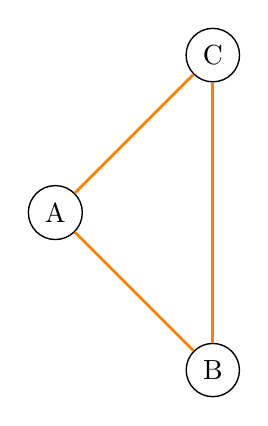
\begin{tikzpicture}[>=latex']
 \SetUpEdge[lw         = 1pt,
            color      = orange,
            labelcolor = red!30,
            labelstyle = {draw,sloped}]
  \tikzset{node distance = 2cm}
  \GraphInit[vstyle=Normal]
  \Vertex[x=-3, y=0]{A}
  \Vertex[x=-1, y=-2]{B}
  \Vertex[x=-1, y=2]{C}
  \tikzset{EdgeStyle/.style={-}}
  \Edge[](A)(B)
  \Edge[](A)(C)
  \Edge[](B)(C)
\end{tikzpicture}
\end{center}
\vspace*{7mm}
Il n'y a plus de réduction possible, on applique donc l'algorithme. Ici, le graphe est un simple triangle. Quelque soit le choix du sommet retiré, les sous-graphes générés seront isomorphes. On se contentera de dérouler une seule branche.\\
On choisit l'arête (A,B):\\
Quelque soit le sommet, prenons A par exemple, le problème sera réduit à VC(G',1), avec G' le graphe :\\
\begin{center}
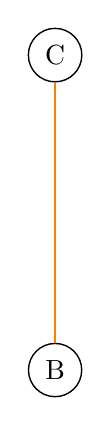
\begin{tikzpicture}[>=latex']
 \SetUpEdge[lw         = 1pt,
            color      = orange,
            labelcolor = red!30,
            labelstyle = {draw,sloped}]
  \tikzset{node distance = 2cm}
  \GraphInit[vstyle=Normal]
  \Vertex[x=-1, y=-2]{B}
  \Vertex[x=-1, y=2]{C}
  \tikzset{EdgeStyle/.style={-}}
  \Edge[](B)(C)
\end{tikzpicture}
\end{center}
\vspace*{7mm}
En procédant de la même manière, on obtient un graphe sans arête à l'itération suivante, qui renvoie donc vrai.\\
\end{enumerate}

\item VC(G2,2)=faux\\
\begin{enumerate}
\item Graphe G2
\begin{center}
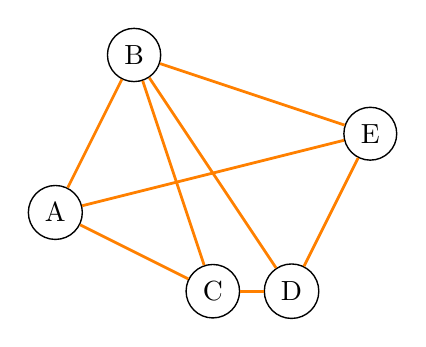
\begin{tikzpicture}[>=latex']
 \SetUpEdge[lw         = 1pt,
            color      = orange,
            labelcolor = red!30,
            labelstyle = {draw,sloped}]
  \tikzset{node distance = 2cm}
  \GraphInit[vstyle=Normal]
  \Vertex[x=-2, y=-1]{A}
  \Vertex[x=-1, y=1]{B}
  \Vertex[x=0, y=-2]{C}
  \Vertex[x=1, y=-2]{D}
  \Vertex[x=2, y=0]{E}
  \tikzset{EdgeStyle/.style={-}}
  \Edge[](A)(B)
  \Edge[](A)(C)
  \Edge[](B)(C)
  \Edge[](C)(D)
  \Edge[](B)(D)
  \Edge[](D)(E)
  \Edge[](A)(E)
  \Edge[](B)(E)
\end{tikzpicture}
\end{center}
\vspace*{7mm}
\item Réductions :\\
\vspace*{7mm}
\begin{center}
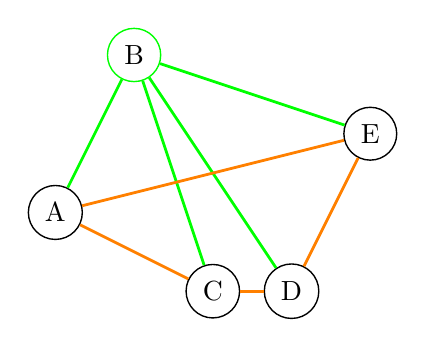
\begin{tikzpicture}[>=latex']
 \SetUpEdge[lw         = 1pt,
            color      = orange,
            labelcolor = red!30,
            labelstyle = {draw,sloped}]
  \tikzset{node distance = 2cm}
  \GraphInit[vstyle=Normal]
  \Vertex[x=-2, y=-1]{A}
  \begin{scope}[VertexStyle/.append style = {draw=green}]
  \Vertex[x=-1, y=1]{B}
  \end{scope}
  \Vertex[x=0, y=-2]{C}
  \Vertex[x=1, y=-2]{D}
  \Vertex[x=2, y=0]{E}
  \tikzset{EdgeStyle/.style={-}}
  \Edge[color=green](A)(B)
  \Edge[](A)(C)
  \Edge[color=green](B)(C)
  \Edge[](C)(D)
  \Edge[color=green](B)(D)
  \Edge[](D)(E)
   \Edge[](A)(E)
  \Edge[color=green](B)(E)
\end{tikzpicture}
\end{center}
\vspace*{7mm}
E est un sommet de degré 4, donc supérieur à k. On le retire donc du graphe. On souhaite désormais connaitre VC(G$\backslash\{E\}$,1).\\
\begin{center}
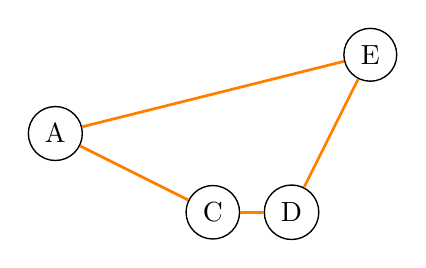
\begin{tikzpicture}[>=latex']
 \SetUpEdge[lw         = 1pt,
            color      = orange,
            labelcolor = red!30,
            labelstyle = {draw,sloped}]
  \tikzset{node distance = 2cm}
  \GraphInit[vstyle=Normal]
  \Vertex[x=-2, y=-1]{A}
  \Vertex[x=0, y=-2]{C}
  \Vertex[x=1, y=-2]{D}
  \Vertex[x=2, y=0]{E}
  \tikzset{EdgeStyle/.style={-}}
  \Edge[](A)(C)
  \Edge[](C)(D)
  \Edge[](D)(E)
   \Edge[](A)(E)
\end{tikzpicture}
\end{center}
\vspace*{7mm}
Il n'y a plus de réduction possible, on applique donc l'algorithme. Ici, on peut remarquer qu'aucun sommet ne couvre toutes les arêtes du graphe, alors que k = 1. Quelque soit le sommet choisi, l'algorithme renverra faux. On se contentera de dérouler une seule branche.\\
On choisit l'arête (A,C):\\
Quelque soit le sommet, prenons A par exemple, le problème sera réduit à VC(G',0), avec G' le graphe :\\
\begin{center}
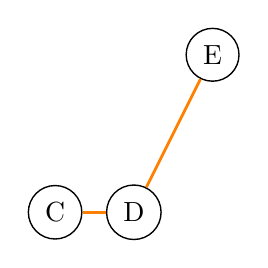
\begin{tikzpicture}[>=latex']
 \SetUpEdge[lw         = 1pt,
            color      = orange,
            labelcolor = red!30,
            labelstyle = {draw,sloped}]
  \tikzset{node distance = 2cm}
  \GraphInit[vstyle=Normal]
  \Vertex[x=0, y=-2]{C}
  \Vertex[x=1, y=-2]{D}
  \Vertex[x=2, y=0]{E}
  \tikzset{EdgeStyle/.style={-}}
  \Edge[](C)(D)
  \Edge[](D)(E)
\end{tikzpicture}
\end{center}
\vspace*{7mm}
Il reste des sommets non couverts et k=0, l'algorithme renvoie donc faux à l'itération suivante.\\
\end{enumerate}
\end{enumerate}
\end{enumerate}

\subsection{Partie calculabilité}



\subsubsection{Exercice 7}

\noindent\fbox{\parbox{\linewidth-2\fboxrule-2\fboxsep}{ \begin {enumerate} \scriptsize  
\item \textbf{Comment enumérer les couples d'entiers?}\\
\item \textbf{Donner les fonctions de codage et de décodage f\oldstylenums{1} $\rightarrow$ x et f\oldstylenums{2} $\rightarrow$ y}\\
\item \textbf{Montrer que l'on peut coder les triplets. Géneraliser aux k-uplets.}\\
\item \textbf{Pensez-vous que l'on peut coder les éléments de l'intervalle [0,1]. Justifier.}
\end{enumerate} }}\\\\

\begin{enumerate}
\item Soit (x,y) $\in$ $\mathbb{N}$ * $\mathbb{N}$, alors faire x + y et trier par ordre lexicographique
\item La fonction de codage est : \[z = \frac{(x+y)(x+y+1)}{2} + y\]\\
Pour les fonction de décodage, posons t tel que \[t = x + y\]
On va prendre t tel que si t augmente de 1 alors \[\frac{t(t+1)}{2} > z\] sinon on a \[\frac{t(t+1)}{2} \le z\]
La fonction de décodage de y est: \[z =\frac{t(t+1)}{2} + y\] \[y = z - \frac{t(t+1)}{2}\]
La fonction de décodage de x est: \[x = t - y\] \[x = -z + t + \frac{t(t+1)}{2}\] \[x = -z + \frac{t(t+3)}{2}\]
\item Pour coder les triplets, il suffit de coder deux entiers et coder le résultat et le dernier entier. 
  \[h(x,y,z)=c(x , c(y,z))\]
On peut répéter ce raisonnement pour les k-uplets, ainsi on a 
\[k(x\oldstylenums{1},x\oldstylenums{2}... x\oldstylenums{k}) = c(x\oldstylenums{1} , c(x\oldstylenums{2} , ... c(x\oldstylenums{k-1},x\oldstylenums{k}))\]
\item On ne peut pas coder les éléments de l'intervalle [0,1] car l'ensemble n'est pas dénombrable. On utilise la diagonale de cantor sur cet ensemble.\\
Supposons que l'on puisse numéroter $\mathbb{N}$  $\rightarrow$ [0,1] et on en définit la suite S telle que tout élément de [0,1] soit élément de la suite S.
Et on définit un réel r tel que la partie entière est égale à 0 et que chaque décimale en position n est égale à sn(n)\footnote{la nème décimale du nème élément de S}+1 si sn(n) est différent de 9 et sn(n)-1 si sn(n) est égal à 9.\\
Par construction, r n'est pas dans S sinon on aurait un Sn tel que \[Sn(n)=r(n)=Sn(n)+1\] ou \[Sn(n)=r(n)=Sn(n)-1\] C'est absurbe, ainsi ce n'est pas dénombrable. 
   
  
\end{enumerate}




\subsubsection{Exercice 8}
\begin{enumerate}
\item Les fonctions primitives récursives sont toutes les fonctions que l'on peut construire à partir des fonctions de base par composition et récursion primitive.\\

  Exemple\\ \\
Soit les fonctions primitives: \\
O $\in \mathbb{N}^0$, $\pi_i^k \in \mathbb{N}^k$ et SUC $\mathbb{N}^1$ 

 \[O() = 0 \] 
\[\pi_i^k(x_1,x_2...,x_k) = x_i \] 
\[SUC(x_1) = x_1 + 1 \] 

Soit la fonction qu'on utilise pour la récursion primitive:\\
g $\in \mathbb{N}^1$
\[g() = SUC(O()) \]

Soit la fonction recursive primitive:\\
f $\in \mathbb{N}^1$
\[f(0) = g()\]
\[f(SUC(n)) = \pi_1^2(f(n),n)\]
  
\item  Question non traitée.\\ 
\item \begin{enumerate}\item Soit la fonction somme définie ainsi:\\
 Sum $\in \mathbb{N}^2$ 
\[Sum(0,y) = \pi_1^1(y) = y \]
\[Sum(Suc(x),y) = \pi_2^3(x,Sum(x,y),y)\]
\item Soit la fonction Mult définie ainsi: \\
Mult $\in \mathbb{N}^2$
\[Mult(O,y) = 0() = 0\]
\[Mult(1,y) = \pi_1^1(y) = y\]
\[Mult(Suc(x),y) = \pi_2^3(x,Sum(Mult(x,y),y),y)\]
\item Soit la fonction puissance définie aisni:\\
 $X^Y$ $\in \mathbb{N}^2$
\[X^Y(x,0) = Suc(0()) = 1\]
\[X^Y(x,Suc(y)) = \pi_2^3(x,Mult(X^Y(x,y),x),y)\]
\item Soit la fonction prédecesseurs telle que: \\
Pred $\in \mathbb{N}^1$
\[Pred(0) = O() = 0\]
\[Pred(Suc(x)) = \pi_1^2(x,Pred(x))\]
\item Soit la fonction soustraction telle que:\\
X-Y $\in \mathbb{N}^2$
\[X-Y(0,y) = 0() = 0\]
\[X-Y(x,0) = \pi_1^1(x) = x\]
\[X-Y(x,y) = \pi_2^3(x,X-Y(Pred(x),Pred(y)),y))\]
\item Soit la fonction sg telle que:
sg $\in \mathbb{N}^1$
\[sg(0) = 0() = 0\]
\[sg(Suc(x)) = \pi_1^2(1,Suc(x))\]
\item Soit la fonction X > Y telle que :\\
X>Y $\in \mathbb{N}^2$
\[X>Y(0,y) = 0\]
\[X>Y(x,0) = 1\]
\[X>Y(x,y) = \pi_2^3(x,X>Y(Pred(x),Pred(y)),y)\]
Soit la fonction X $\ge$ Y telle que :\\
X$\ge$Y $\in \mathbb{N}^2$
\[X\ge Y(0,0) = 1\]
\[X\ge Y(0,y) = 0\]
\[X\ge Y(x,0) = 1\]
\[X\ge Y(x,y) = \pi_2^3(x,X>Y(Pred(x),Pred(y)),y)\]

\end{enumerate}
\item \begin{enumerate} 

\item Voici la fonction d'Ackerman pour 0 $\le$ m $\le$ 3 et 0 $\le$ n $\le$ 4 \\
\begin{center}
\begin{tabular}{| c || c | c | c | c | c |}
\hline
m/n & 0 & 1 & 2 & 3 & 4 \\
\hline
\hline
0 & 1 & 2 & 3 & 4 & 5 \\
\hline
1 & 2 & 3 & 4 & 5 & 6 \\
\hline
2 & 3 & 5 & 7 & 9 & 11 \\
\hline
3 & 5 & 13 & 28 & 58 & 118 \\
\hline
\end{tabular}
\end{center}

\item Faisons une preuve par récurrence
\[A_0(n) = Suc(n) = n + 1\]
Hypothèse: A\tiny m\normalsize (n) est primitive récursive\\
Montrons que A\tiny m+1\normalsize (n) est primitive récursive\\ 

Si n = 0, on a que A\tiny m+1\normalsize (n) = A\tiny m\normalsize (1). D'après l'hypothèse de réccurence, on a que A\tiny m\normalsize (n) est primitive récursive. Donc A\tiny m+1\normalsize (n) est primitf récursive\\

Si n > 0, on a que A\tiny m+1\normalsize (n) = A\tiny m\normalsize (A\tiny m+1\normalsize (n)).\\
Posons n' = A\tiny m+1\normalsize (n). Donc on a A\tiny m\normalsize (n'). D'après l'hypothèse de récurrence, on a que A\tiny m\normalsize (n) est primitive récursive pour tous n $\in \mathbb{N}$ . Donc A\tiny m+1\normalsize (n) est primitif récursive.\\

\item 
Faisons une preuve par récurrence 
\[A_0(n) = n+1 \] 
n+1 > n donc c'est vrai au premier rang\\
Hypothèse: A\tiny m\normalsize (n) > n \\
Montrons que A\tiny m+1\normalsize (n) > n\\ \\
Maitenant, on applique une récurrence sur n\\
n = 0 : A\tiny m+1\normalsize (1) > 1  > 0
Hypothèse: A\tiny m+1\normalsize (n) > n \\
Montrons que: A\tiny m+1\normalsize (n+1) > n+1\\
On utilise les deux hypothèse de récurrence:\\
\[A\tiny m+1\normalsize (n+1) = A\tiny m\normalsize (A\tiny m+1\normalsize (n)) > A\tiny m+1\normalsize (n) > n \]
Ainsi \[A\tiny m+1\normalsize (n) \ge n+1\]
Donc \[A\tiny m+1\normalsize (n+1) > n+1\]
On peux donc conclure que A\tiny m\normalsize (n) > n\\

\item  Il faut montrer que A\tiny m+1\normalsize (n) - A\tiny m\normalsize (n)  $\ge$ 0\\
Faisons une preuve par récurrence sur m \\
\[A_0(n+1) - A_0(n) = n + 1 - n = 1\] 
Hypothèse: A\tiny m\normalsize (n+1) - A\tiny m\normalsize (n) > 0\\
Montrons que A\tiny m+1\normalsize (n+1) - A\tiny m+1\normalsize (n) > 0\\
A\tiny m+1\normalsize (n+1) = A\tiny m\normalsize (A\tiny m+1\normalsize (n)) > A\tiny m\normalsize (n)\\
On peut conclure que\\ 
A\tiny m\normalsize (n+1) - A\tiny m\normalsize (n) > 0

\item 
Pour n = 0: A\tiny m+1\normalsize (0) = A\tiny m\normalsize (1). De plus, d'après la question précédente, on a que A\tiny m\normalsize (1) > A\tiny m\normalsize (0)\\\\
Pour n > 0: A\tiny m+1\normalsize (n) = A\tiny m\normalsize (A\tiny m+1\normalsize (n-1)). De plus on a que A\tiny m\normalsize (n-1) > n - 1 $\rightarrow$ A\tiny m\normalsize (n-1) $\ge$ n\\
Comme la fonction est strictement croissante, on a que  A\tiny m\normalsize (A\tiny m\normalsize (n-1)) $\ge$ A\tiny m\normalsize (n) \\ \\
On peux en conclure que \\
A\tiny m+1\normalsize (n) = A\tiny m\normalsize (A\tiny m+1\normalsize (n-1)) $\ge$ A\tiny m\normalsize (n) 

\item D'après les questions précédentes, on a montré que A\tiny m+1\normalsize (n) $\ge$ A\tiny m\normalsize (n) et que A\tiny m\normalsize (n+1) > A\tiny m\normalsize (n). Ceci prouve que $A_m^k$ est strictement croissante. 

\item Faisons une preuve pas récurrence sur k.\\
Au cas de base, on a bien $A_{m+1}$\normalsize (n) $\ge$ $A_m$\normalsize (n)\\
Hypothèse: $A_{m+1}$\normalsize (n + k) $\ge$ $A^k_m$\normalsize (n)\\
Montrons que : $A_{m+1}$(n + k + 1) $\ge$ $A^{k+1}_m$(n)\\
D'après l'hypothèse de récurrence, on a \\
\[A^{k+1}_m = A_m(A^k_m(n)) \le A_m(A_{m+1}(n + k))\] 
De plus:\\
\[A_{m+1}(n + k + 1) = A_m(A_{m+1}(n + k))\]
On peut conclure que:\\
\[A^{k+1}_m = A_m(A^k_m(n)) \le A_{m+1}(n + k + 1)\]
\item 
Faisons une preuve par l'absurbe, soit la fonction d'Ackermann primitive récursive.\\\\
Sois la fonction \[f: \mathbb{N} \rightarrow \mathbb{N} : n \rightarrow A(n,2n)\]
Comme la fonction d'Ackerman est primitive récursive alors f est primitive récursive.   

\end{enumerate}

\end{enumerate}

\end{document}